% =====================================================================
% ELE637 -- Pensamento Sistêmico em Engenharia -- Trabalho Prático (Grupo 3)
% Slides no formato das aulas: Beamer, 16:9, tema Madrid em vermelho UFMG
% =====================================================================
\documentclass[aspectratio=169, 10pt]{beamer}

\usepackage[utf8]{inputenc}
\usepackage[T1]{fontenc}
\usepackage[brazil]{babel}
\usepackage{amsmath, amssymb}
\usepackage{booktabs}
\usepackage{tikz}
\usepackage{graphicx}
% figuras próprias em figuras/; gráficos lidos direto de ../outputs
\graphicspath{{figuras/}{../outputs/}}
\usepackage[authoryear, round]{natbib}

% ---------------------------------------------------------------- tema
\usetheme{Madrid}
\definecolor{ufmgred}{RGB}{200,16,46}
\definecolor{blocoazul}{RGB}{0,74,117}
\definecolor{blocoverde}{RGB}{0,96,0}
\usecolortheme[named=ufmgred]{structure}
\setbeamercolor{block title}{bg=blocoazul, fg=white}
\setbeamercolor{block body}{bg=blocoazul!10, fg=black}
\setbeamercolor{block title example}{bg=blocoverde, fg=white}
\setbeamercolor{block body example}{bg=blocoverde!10, fg=black}
\setbeamercolor{block title alerted}{bg=ufmgred, fg=white}
\setbeamercolor{block body alerted}{bg=ufmgred!10, fg=black}
\setbeamertemplate{navigation symbols}{}
\setbeamertemplate{itemize items}[circle]
\setbeamertemplate{enumerate items}[default]

% fonte da figura ou do dado, no rodapé do slide (como nas aulas)
\newcommand{\fonte}[1]{%
  \begin{tikzpicture}[remember picture, overlay]
    \node[anchor=south west, font=\tiny, text width=0.9\paperwidth]
      at ([xshift=4pt, yshift=12pt]current page.south west) {#1};
  \end{tikzpicture}}

% slide de seção: caixa vermelha centralizada
\AtBeginSection[]{%
  \begin{frame}[plain, noframenumbering]
    \vfill\centering
    \begin{beamercolorbox}[sep=10pt, center, rounded=true, shadow=true]{title}
      \usebeamerfont{title}\insertsectionhead
    \end{beamercolorbox}
    \vfill
  \end{frame}}

% ---------------------------------------------------------------- capa
\title[Pensamento Sistêmico em Engenharia]{Dinâmica dos desvios ambientais por falha humana}
\subtitle{Pressão operacional, supervisão e moral coletiva}
\author[Grupo 3]{%
  Elias Daniel Moreira de Siqueira \and Henrique Viana Lima de Oliveira\\
  Pedro Armando Oliveira Duarte \and Rafael Campello Soares}
\institute[UFMG]{ELE637 -- Pensamento Sistêmico em Engenharia\\
  Escola de Engenharia -- Universidade Federal de Minas Gerais}
\date[Desvios ambientais]{}
\titlegraphic{%
  
\includegraphics[height=0.9cm]{figuras/logo_ufmg.png}\hspace{6cm}%
  
\includegraphics[height=0.9cm]{figuras/logo_engenharia.png}}

\begin{document}

\begin{frame}[plain]
  \titlepage
\end{frame}

\begin{frame}{Sumário}
  \tableofcontents
\end{frame}

% =====================================================================
\section{A situação estudada}
% =====================================================================

\begin{frame}{A situação estudada}{Desvios ambientais por falha humana}
  \begin{columns}[T]
    \begin{column}{0.48\textwidth}
      \begin{block}{Origem}
        Melhoria contínua na área ambiental da Vallourec: estruturas e procedimentos para prevenir desvios causados por falha humana.
      \end{block}
      \begin{itemize}
        \item \textbf{Leves:} desorganização, sujeira, lixo comum no lugar errado. Frequentes e negligenciados.
        \item \textbf{Médios:} exigem contingência e ação corretiva.
        \item \textbf{Graves:} vazamento químico, emissões. Multa, impacto severo, risco de embargo.
      \end{itemize}
      \small Desvios leves frequentes normalizam os mais sérios \citep{banja2010}.
    \end{column}
    \begin{column}{0.48\textwidth}
      \begin{exampleblock}{Comportamento observado}
        Crônico: os desvios nunca somem. Picos em períodos de maior produção, queda depois de campanhas e retorno gradual ao nível anterior.
      \end{exampleblock}
      \begin{alertblock}{Pergunta}
        Como pressão, supervisão e moral interagem para que os desvios se estabilizem em nível baixo ou escalem para a desordem? Quais alavancas reduzem o erro?
      \end{alertblock}
    \end{column}
  \end{columns}
\end{frame}

\begin{frame}{A situação estudada}{Causas-raiz e sinais de complexidade}
  \begin{columns}[T]
    \begin{column}{0.48\textwidth}
      \begin{block}{Três causas-raiz (relato do integrante)}
        \begin{enumerate}
          \item \textbf{Pressão operacional:} sem tempo, o resíduo fica no local mais próximo.
          \item \textbf{Complexidade fabril:} dezenas de tipos produtos químicos, volume de padrões operacionais e produtos distintos, além de um ambiente em constante mudança.
          \item \textbf{Desengajamento:} mesmo sem pressão e conhecendo a regra, há quem não se importe.
        \end{enumerate}
      \end{block}
      \small\textbf{Fronteira:} dentro, trabalhadores, supervisão, pressão, moral, desordem visível e prejuízo; fora, legislação, falhas de equipamento e desvios não humanos.
    \end{column}
    \begin{column}{0.48\textwidth}
      \begin{exampleblock}{Sinais de complexidade}
        \begin{itemize}
          \item Não linearidade e limiar: a norma pode colapsar
          \item Emergência: ordem ou desordem a partir de vizinhos
        \end{itemize}
      \end{exampleblock}
    \end{column}
  \end{columns}
\end{frame}

% =====================================================================
\section{Modelo conceitual}
% =====================================================================

\begin{frame}{Modelo conceitual}{Diagrama de Loop Causal}
  \begin{columns}[c]
    \begin{column}{0.56\textwidth}
      \centering
      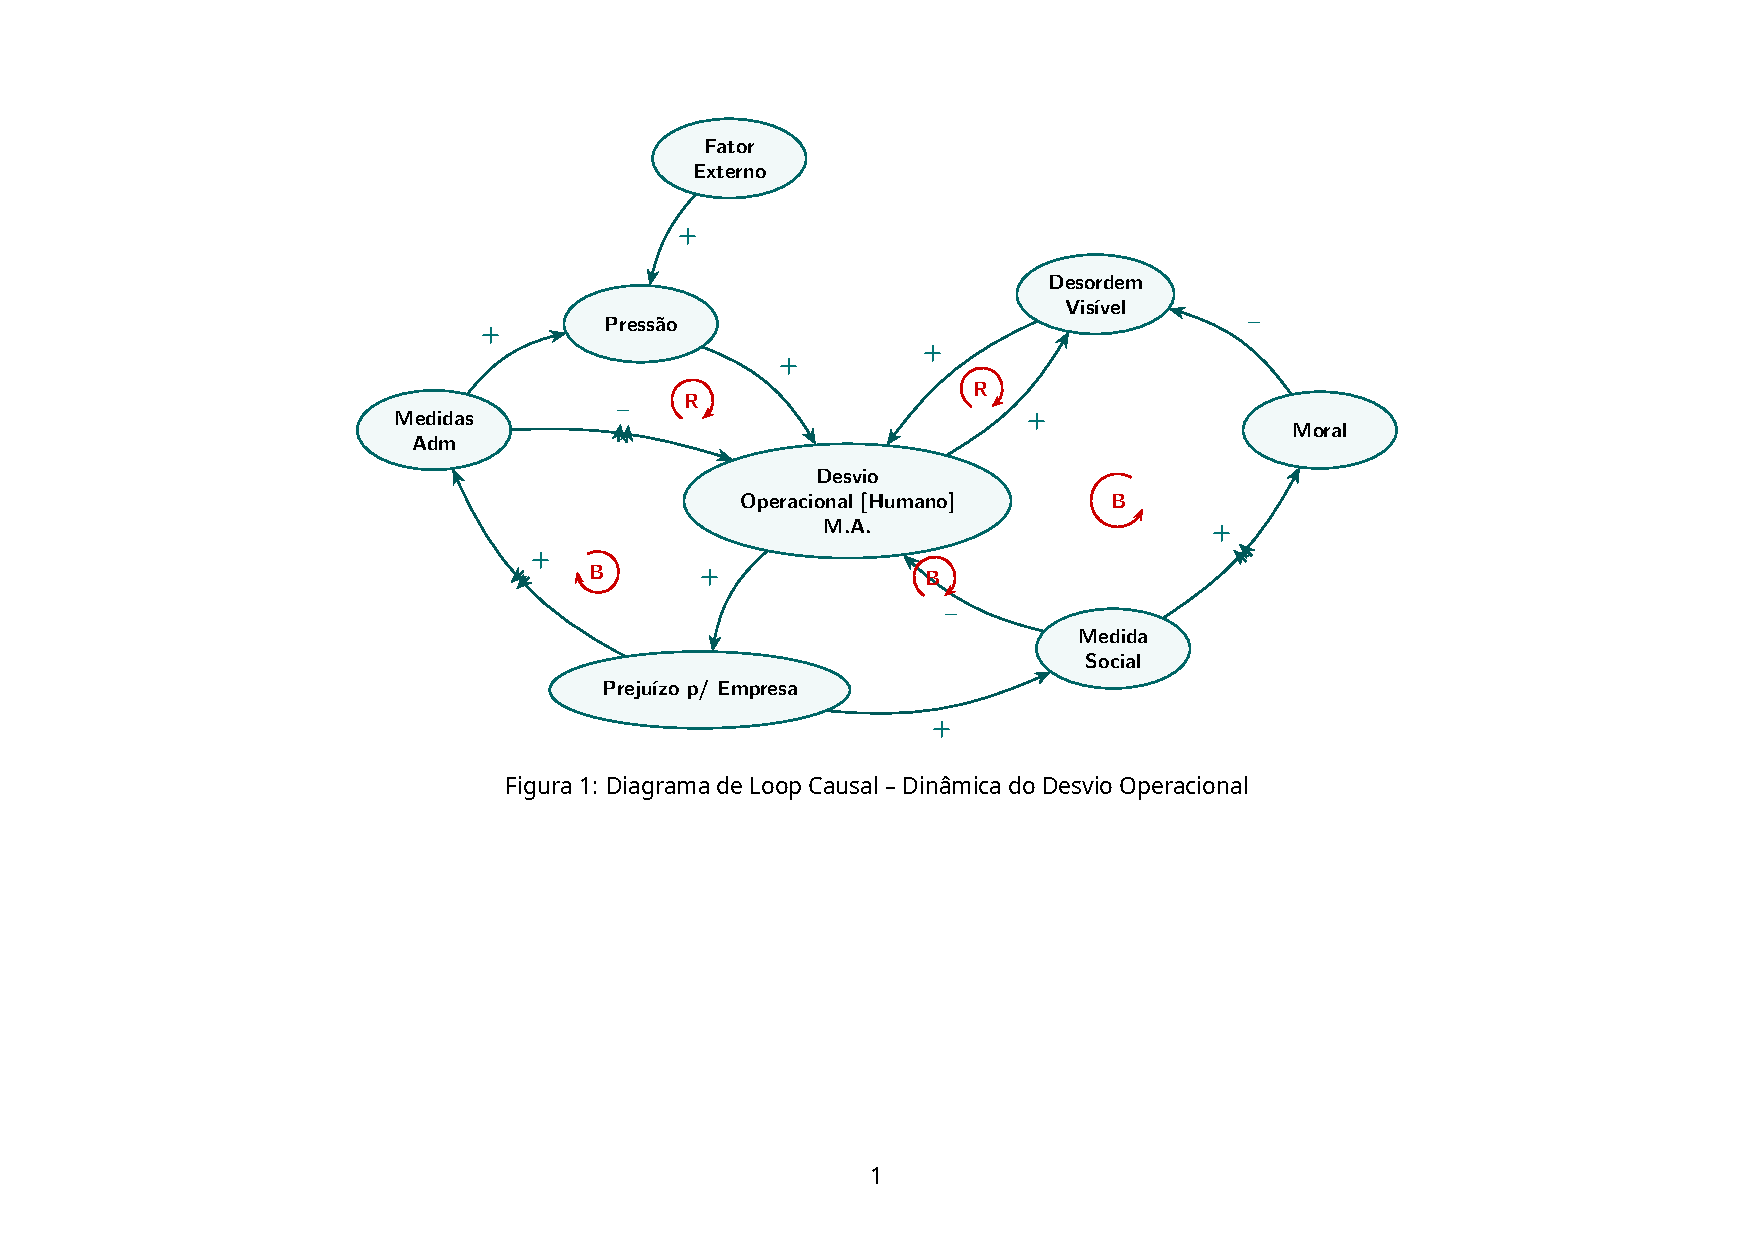
\includegraphics[trim=160pt 235pt 160pt 50pt, clip, width=\textwidth]{figuras/diagrama_loop_causal.pdf}
    \end{column}
    \begin{column}{0.42\textwidth}
      \small
      \begin{itemize}
        \item \textbf{R1} desordem visível: ver erro por perto aumenta o erro (janelas quebradas)
        \item \textbf{R2} resistência a políticas: Prejuizo p/ Empresa\ $\rightarrow$ medida adm.\ $\rightarrow$ pressão $\rightarrow$ desvio
        \item \textbf{B1} supervisão: medida adm.\ reduz o desvio, com atraso
        \item \textbf{B2} medida social imediata: o funcionário corrige o desvio na hora e dá \emph{feedback}
        \item \textbf{B3} moral: palestras e eventos $\rightarrow$ moral $\rightarrow$ menos desordem, com atraso
      \end{itemize}
      Traços duplos indicam atrasos.
    \end{column}
  \end{columns}
  \fonte{\citet{ball2012}.}
\end{frame}

\begin{frame}{Modelo conceitual}{Cada laço em números}
  \centering\footnotesize
  Trabalhador médio ($M=0{,}5$; $P=0{,}5$; $D=0$; $S=0$): erra \textbf{8,3\%} por hora, ou seja, um erro a cada 12 h por pessoa e $\approx$10 erros por hora em 120 trabalhadores.\\[6pt]
  \begin{tabular}{@{}llp{4.2cm}p{4.6cm}@{}}
    \toprule
    Laço & Tipo & Exemplo & Probabilidade de erro \\
    \midrule
    R1 & Reforço & Resíduo visível nas células vizinhas & $D=0{,}5$: 15,4\%; $D=1$: 26,9\% \\
    R2 & Reforço & Cobrança de metas após um prejuízo & $P=1$: 14,2\%; $P=0$: 4,7\% \\
    B1 & Balanceamento & Supervisor presente no entorno & $S=1$: 3,2\% ($-61\%$) \\
    B2 & Balanceamento & Correção imediata e \emph{feedback} no local & agente remove o resíduo com 88\% (trabalhador: 50\%) \\
    B3 & Balanceamento & Palestras e eventos que elevam a moral & $M=0{,}75$: 5,2\%; $M=0{,}25$: 13,0\% \\
    \bottomrule
  \end{tabular}
  \fonte{Cálculo pelas equações do modelo computacional.}
\end{frame}

\begin{frame}{Modelo conceitual}{Arquétipo e o que entra no modelo computacional}
  \begin{columns}[T]
    \begin{column}{0.48\textwidth}
      \begin{block}{Relação de atenção (B1 + R2)}
        A medida administrativa reduz a chance de novos desvios, mas só depois de um atraso. Antes desse efeito, a medida gera um pulso de pressão que representa o período de adaptação dos trabalhadores.\\[4pt]
        Passado esse período, a medida administrativa tem o efeito pretendido de reduzir as chances de um novo erro aparecer.
      \end{block}
    \end{column}
    \begin{column}{0.48\textwidth}
      \begin{exampleblock}{Recorte de curto prazo}
        1 passo $\approx$ 1 hora; 600 passos $\approx$ algumas semanas.\\[4pt]
        \textbf{Simulado diretamente:} R1, correção e supervisão em campo.\\[4pt]
        \textbf{Como parâmetro:} R2, B1, B2 e B3 têm atrasos de semanas a meses. Pressão $P$ e moral $M$ ficam constantes em cada execução e variam entre execuções.
      \end{exampleblock}
    \end{column}
  \end{columns}
  \fonte{\citet{meadows2022}.}
\end{frame}

% =====================================================================
\section{Modelo computacional}
% =====================================================================

\begin{frame}{Modelo computacional}{Agentes e ambiente}
  \begin{columns}[T]
    \begin{column}{0.52\textwidth}
      \begin{block}{Ambiente}
        Grade $30\times30$ toroidal. Cada célula tem ou não resíduo (desordem visível). No máximo um agente por célula.
      \end{block}
      \begin{itemize}
        \item \textbf{120 trabalhadores:} andam ao acaso, erram e corrigem.
        \item \textbf{8 corretores:} erram menos, corrigem mais e reduzem o erro de quem está a até $r_s=3$ células.
        \item \textbf{Moral individual} $M_i \sim \mathcal{N}(0{,}5;\,0{,}25^2)$
      \end{itemize}
    \end{column}
    \begin{column}{0.44\textwidth}
      \begin{exampleblock}{Cada passo}
        \begin{enumerate}
          \item Percepção de $D_i$ e $S_i$
          \item Erro: resíduo na própria célula
          \item Correção (se erra e corrige, o erro prevalece)
          \item Movimento, em ordem sorteada
        \end{enumerate}
      \end{exampleblock}
      \small Por que ABM: o erro se espalha entre vizinhos, a posição importa e a moral varia de pessoa para pessoa.
    \end{column}
  \end{columns}
  \fonte{\citet{rangoni2017}; \citet{savarimuthu2008}.}
\end{frame}

\begin{frame}{Modelo computacional}{Regras}
  \begin{block}{Probabilidade de erro (trabalhador)}
    \vspace{-8pt}
    \[
      p^{\text{erro}}_i=\sigma\!\left(b_T+\beta_P P+\beta_D D_i(t)-\beta_S S_i(t)-\beta_M M_i\right),
      \qquad \sigma(x)=\frac{1}{1+e^{-x}}
    \]
    \vspace{-10pt}
  \end{block}
  \begin{columns}[T]
    \begin{column}{0.48\textwidth}
      \begin{block}{Correção}
        \vspace{-8pt}
        \[ p^{\text{corr}}_i=\sigma\!\left(c+\gamma\, M_i\right) \]
        \vspace{-12pt}
      \end{block}
      \small
      $D_i$: fração das 8 vizinhas com resíduo.\\
      $S_i=1$ se há corretor a distância $\le r_s$.\\
      Corretor: mesma forma, sem o termo $S_i$.
    \end{column}
    \begin{column}{0.48\textwidth}
      \begin{exampleblock}{Valores de referência ($P=M=0{,}5$, $D=S=0$)}
        \small
        \begin{tabular}{@{}lcc@{}}
          \toprule
          & Trabalhador & Corretor \\
          \midrule
          Erra & 8,3\% & 2,4\% \\
          Corrige & 50\% & 88\% \\
          \bottomrule
        \end{tabular}
      \end{exampleblock}
    \end{column}
  \end{columns}
\end{frame}

\begin{frame}{Modelo computacional}{Políticas de movimento dos corretores}
  \centering\small
  \begin{tabular}{@{}lp{4.6cm}p{4.6cm}c@{}}
    \toprule
    Política & Pontuação da célula candidata & Intenção & Realimentação \\
    \midrule
    Aleatória & Igual para todas & Supervisão sem informação (base) & Não \\
    Reativa & Nº de resíduos a distância $\le r_s$ & Concentrar a supervisão onde o problema já apareceu & Sim \\
    De cobertura & Distância ao corretor mais próximo & Espalhar a supervisão antes que haja desordem & Não \\
    \bottomrule
  \end{tabular}\\[8pt]
  \begin{block}{Como o corretor decide}
    Avalia a própria célula e as vizinhas livres (até 9 candidatas) e vai para a de maior pontuação; com probabilidade $\varepsilon=0{,}1$ anda ao acaso.\\
    Exemplo (reativa, $r_s=3$): janela de $7\times7=49$ células; candidata A com 6 resíduos e B com 2: vai para A.
  \end{block}
\end{frame}

\begin{frame}{Modelo computacional}{Parâmetros ancorados na literatura}
  \centering\small
  \begin{tabular}{@{}llp{8.2cm}@{}}
    \toprule
    Parâmetro & Base & Ancoragem \\
    \midrule
    $b_T$, $b_A$ (erro basal) & $-2{,}0$; $-3{,}0$ & erro de 2--10\% em tarefa rotineira \citep{kirwan1994} \\
    $\beta_P$ (pressão) & 1,2 & efeito pequeno a moderado \citep{szalma2008} \\
    $\beta_D$ (contágio) & 1,4 & desordem dobra o descarte indevido \citep{keizer2008} \\
    $\beta_S$ (supervisão) & 1,0 & observador visível triplica a conformidade \citep{srigley2014} \\
    $\beta_M$ (moral) & 2,0 & clima de segurança prediz conformidade \citep{christian2009} \\
    $c_T$, $c_A$ (correção) & $-1{,}5$; $1{,}0$ & corretores têm papel explícito de limpeza \citep{rangoni2017} \\
    \bottomrule
  \end{tabular}\\[8pt]
  Desordem final = média da fração de células com resíduo nos últimos 50 de 600 passos; IC 95\% sobre 10 a 20 sementes.
\end{frame}

% =====================================================================
\section{Simulação e análise}
% =====================================================================

\begin{frame}{Simulação e análise}{Cenário base}
  \centering
  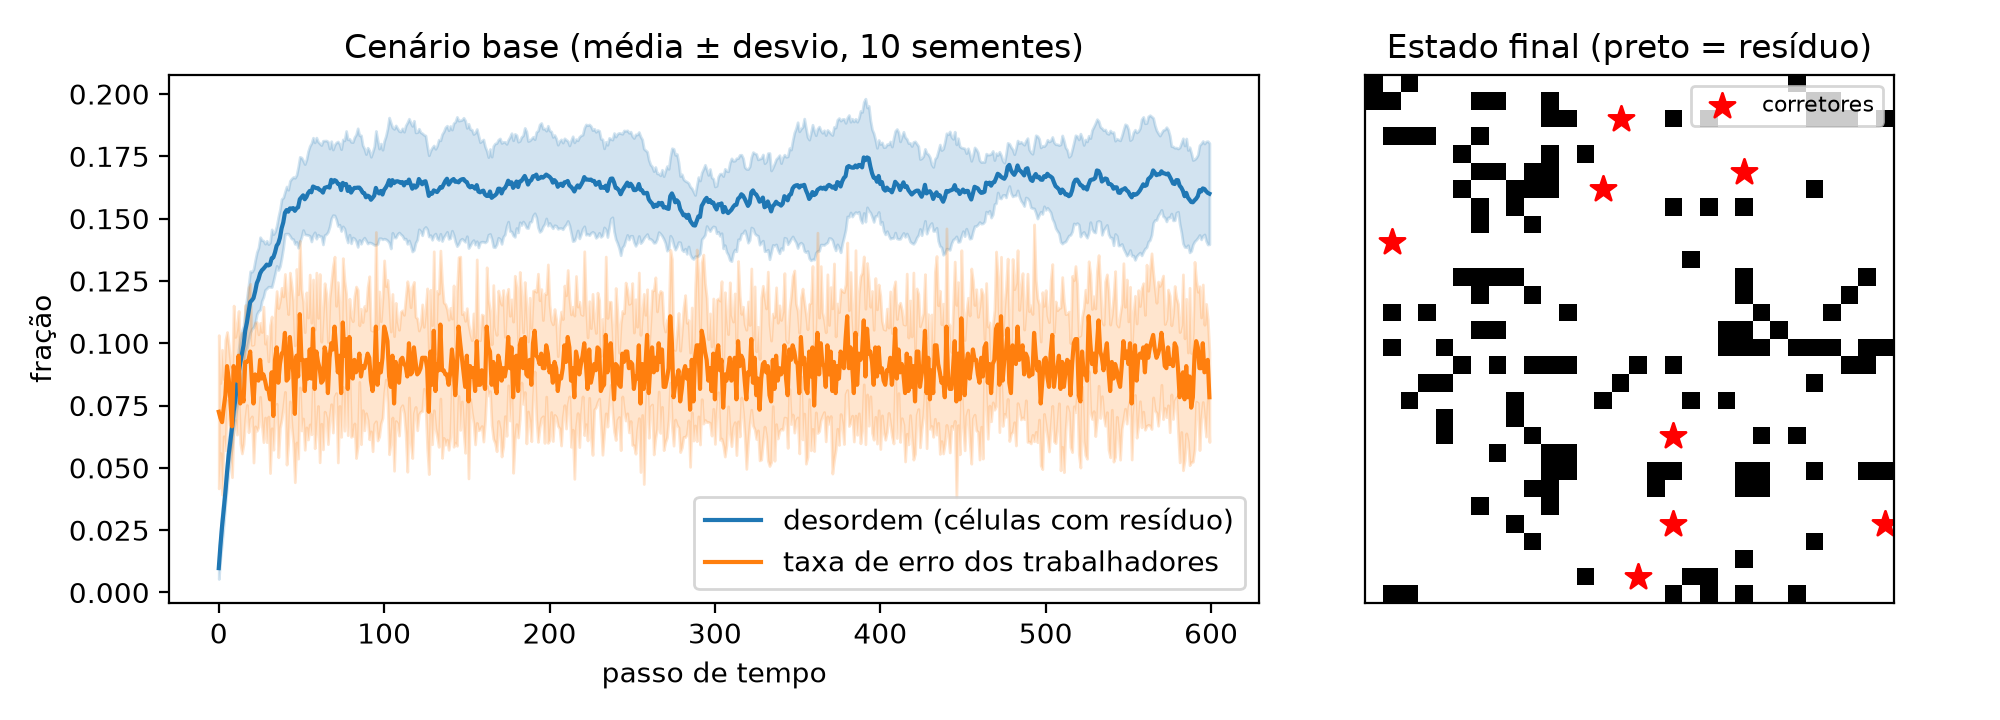
\includegraphics[width=0.74\textwidth]{fig1_cenario_base.png}\\[2pt]
  \small
  \begin{itemize}
    \item Patamar de \textbf{0,160} (IC 95\%: $\pm0{,}009$), cerca de 144 das 900 células; metade em 11 passos e 90\% em 45 passos.
    \item 9,1\% dos trabalhadores erram a cada passo ($\approx$11 descartes por passo).
    \item Mesmo padrão da área: os desvios nunca somem e não explodem.
  \end{itemize}
  \fonte{Média $\pm$ desvio de 10 sementes.}
\end{frame}

\begin{frame}{Simulação e análise}{Valores extremos e choque de pressão}
  \begin{columns}[T]
    \begin{column}{0.5\textwidth}
      \centering
      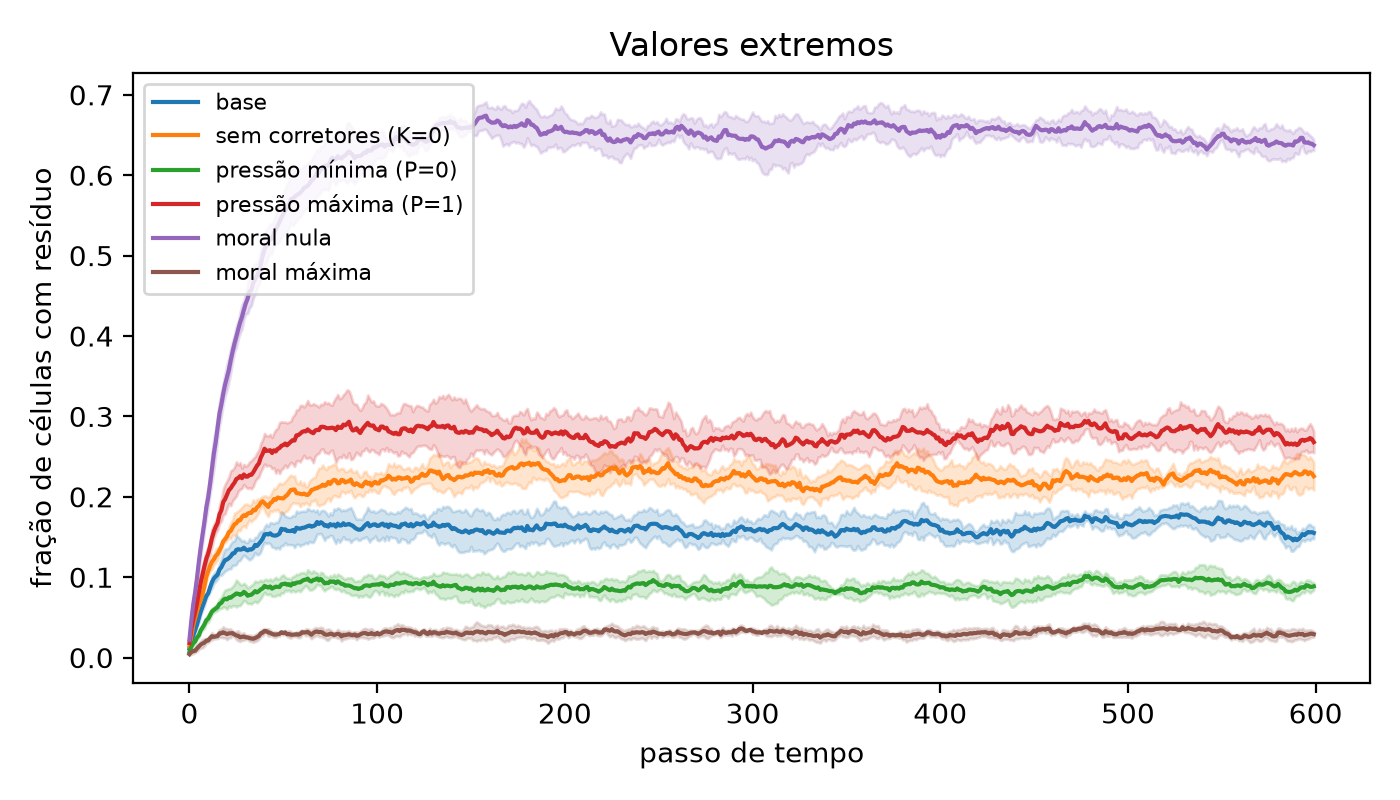
\includegraphics[width=\textwidth]{fig2_extremos.png}
    \end{column}
    \begin{column}{0.5\textwidth}
      \centering
      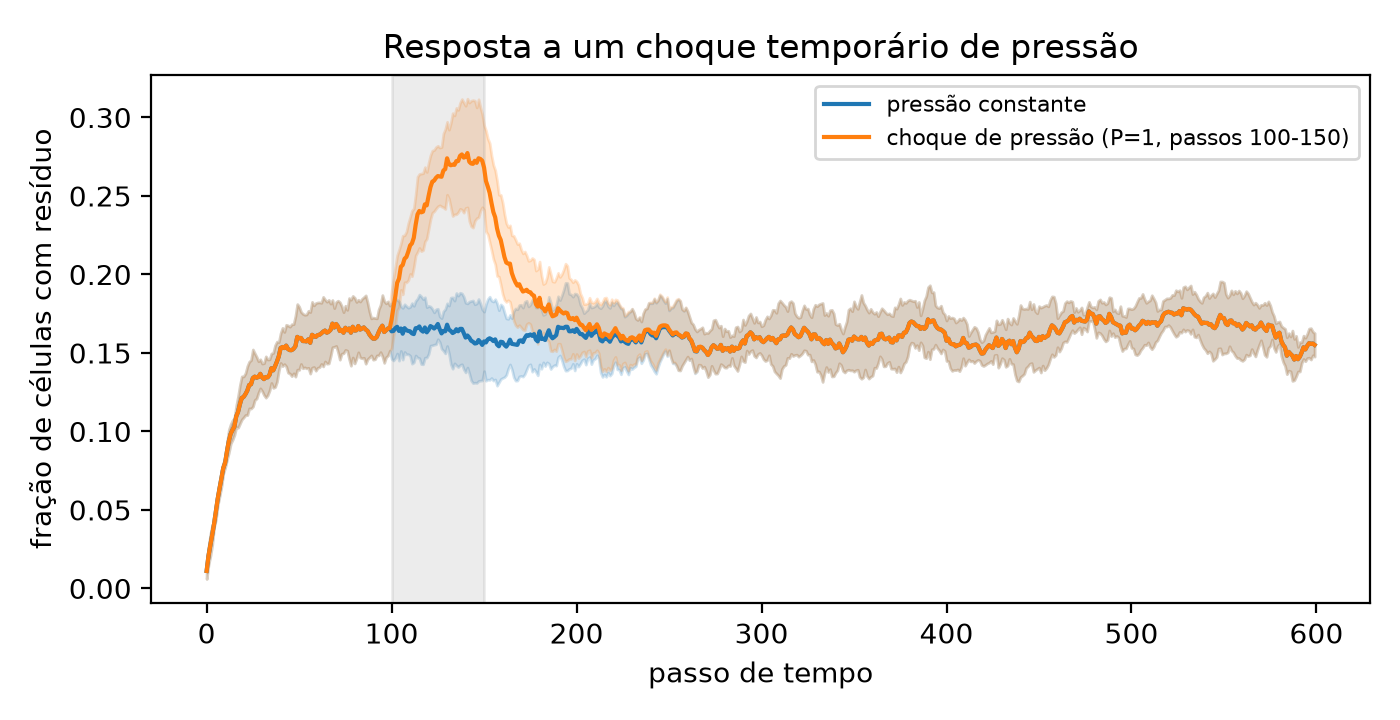
\includegraphics[width=\textwidth]{fig5_choque_pressao.png}
    \end{column}
  \end{columns}
  \vspace{2pt}
  \footnotesize
  \begin{tabular}{@{}lcccccc@{}}
    \toprule
    & moral 1 & $P=0$ & base & $K=0$ & $P=1$ & moral 0 \\
    \midrule
    desordem final & 0,03 & 0,09 & 0,16 & 0,22 & 0,28 & 0,64 \\
    vs.\ base & $-81\%$ & $-44\%$ & --- & $+38\%$ & $+75\%$ & $\times4$ \\
    \bottomrule
  \end{tabular}\hfill
  \begin{minipage}{0.40\textwidth}
    Choque ($P=1$, passos 100--150): 0,16 $\rightarrow$ 0,27 ($+67\%$). Excesso cai pela metade a cada $\approx$10 passos; volta ao base em $\approx$45 passos.
  \end{minipage}
  \fonte{Moral é o parâmetro de maior amplitude (0,61), contra 0,19 da pressão e 0,06 dos corretores.}
\end{frame}

\begin{frame}{Simulação e análise}{Pressão e corretores}
  \begin{columns}[T]
    \begin{column}{0.46\textwidth}
      \centering\small
      \begin{tabular}{@{}cccc@{}}
        \toprule
        & $K=0$ & $K=8$ & $K=16$ \\
        \midrule
        $P=0$ & 0,120 & 0,091 & 0,069 \\
        $P=0{,}5$ & 0,221 & 0,163 & 0,126 \\
        $P=1$ & 0,372 & 0,277 & 0,215 \\
        \bottomrule
      \end{tabular}\\[2pt]
      \scriptsize Desordem final, 10 sementes.
    \end{column}
    \begin{column}{0.52\textwidth}
      \small
      \begin{itemize}
        \item Sem corretores, $P=0\to1$ multiplica a desordem por 3,1.
        \item Os primeiros 8 corretores reduzem 24\% a 26\% em qualquer pressão; o ganho absoluto é 0,095 com $P=1$ contra 0,029 com $P=0$.
        \item 16 corretores com $P=1$ (0,215) equivalem a $K=0$ com $P=0{,}5$ (0,221).
      \end{itemize}
    \end{column}
  \end{columns}
  \vspace{4pt}
  \begin{alertblock}{}
    \centering A supervisão atenua a pressão, mas não a substitui.
  \end{alertblock}
\end{frame}

\begin{frame}{Simulação e análise}{Existe ponto de virada?}
  \begin{columns}[T]
    \begin{column}{0.5\textwidth}
      \centering
      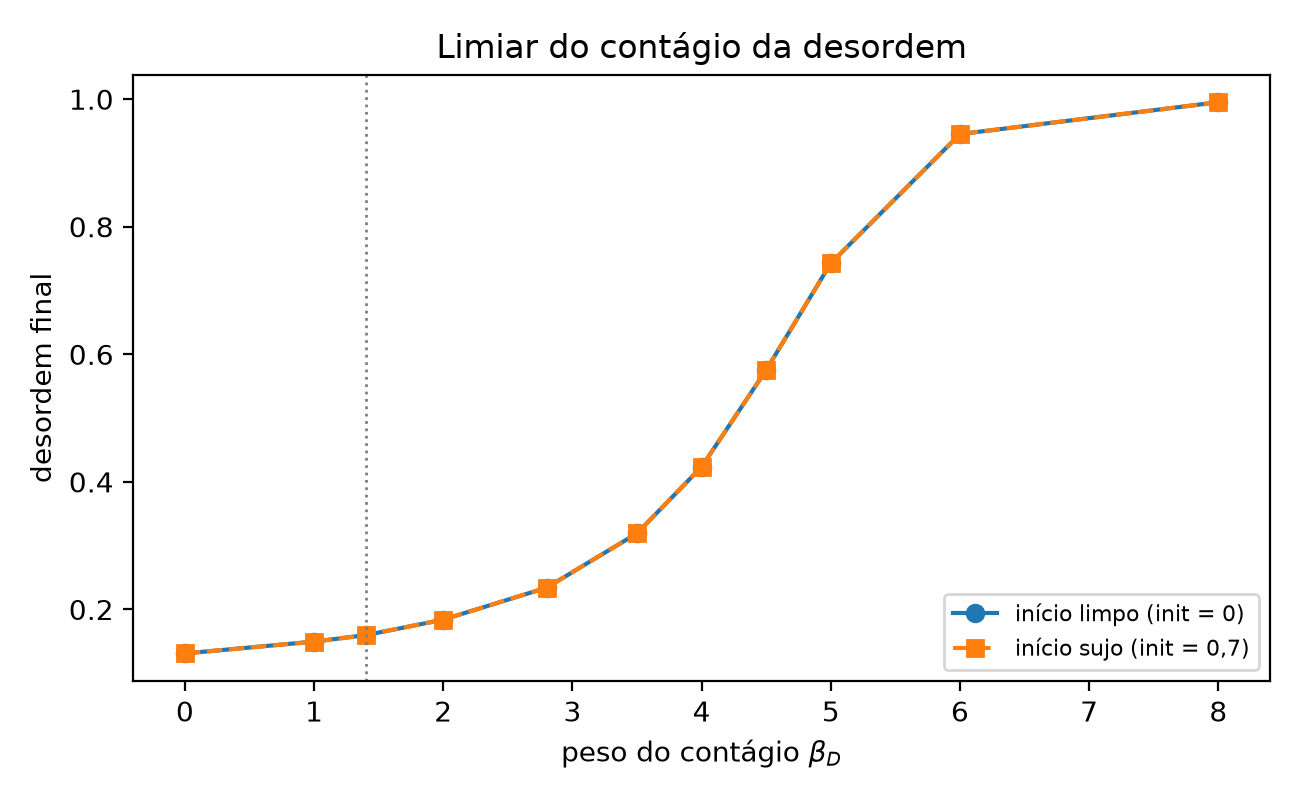
\includegraphics[width=0.95\textwidth]{fig6_limiar_contagio.png}
    \end{column}
    \begin{column}{0.48\textwidth}
      \small
      \begin{itemize}
        \item Início limpo e sujo coincidem: \textbf{um único equilíbrio}, sem histerese.
        \item Até $\beta_D=2{,}8$: 0,131 $\rightarrow$ 0,234 ($\approx$0,04 por unidade).
        \item Entre 4 e 5: 0,424 $\rightarrow$ 0,743 ($\approx$0,32 por unidade, 9 vezes mais rápido).
        \item $\beta_D=6$: 0,945; $\beta_D=8$: 0,995.
        \item Base ($\beta_D=1{,}4$): o contágio responde por 0,029 dos 0,160 (18\%). Duplicar a desordem exige $\beta_D\approx3{,}5$.
      \end{itemize}
    \end{column}
  \end{columns}
  \vspace{4pt}
  \begin{alertblock}{}
    \centering O limiar está no contágio (R1), entre $\beta_D\approx3$ e 5: acima dele a norma colapsa.
  \end{alertblock}
  \fonte{4 sementes por ponto.}
\end{frame}

\begin{frame}{Simulação e análise}{Sensibilidade dos parâmetros incertos}
  \centering
  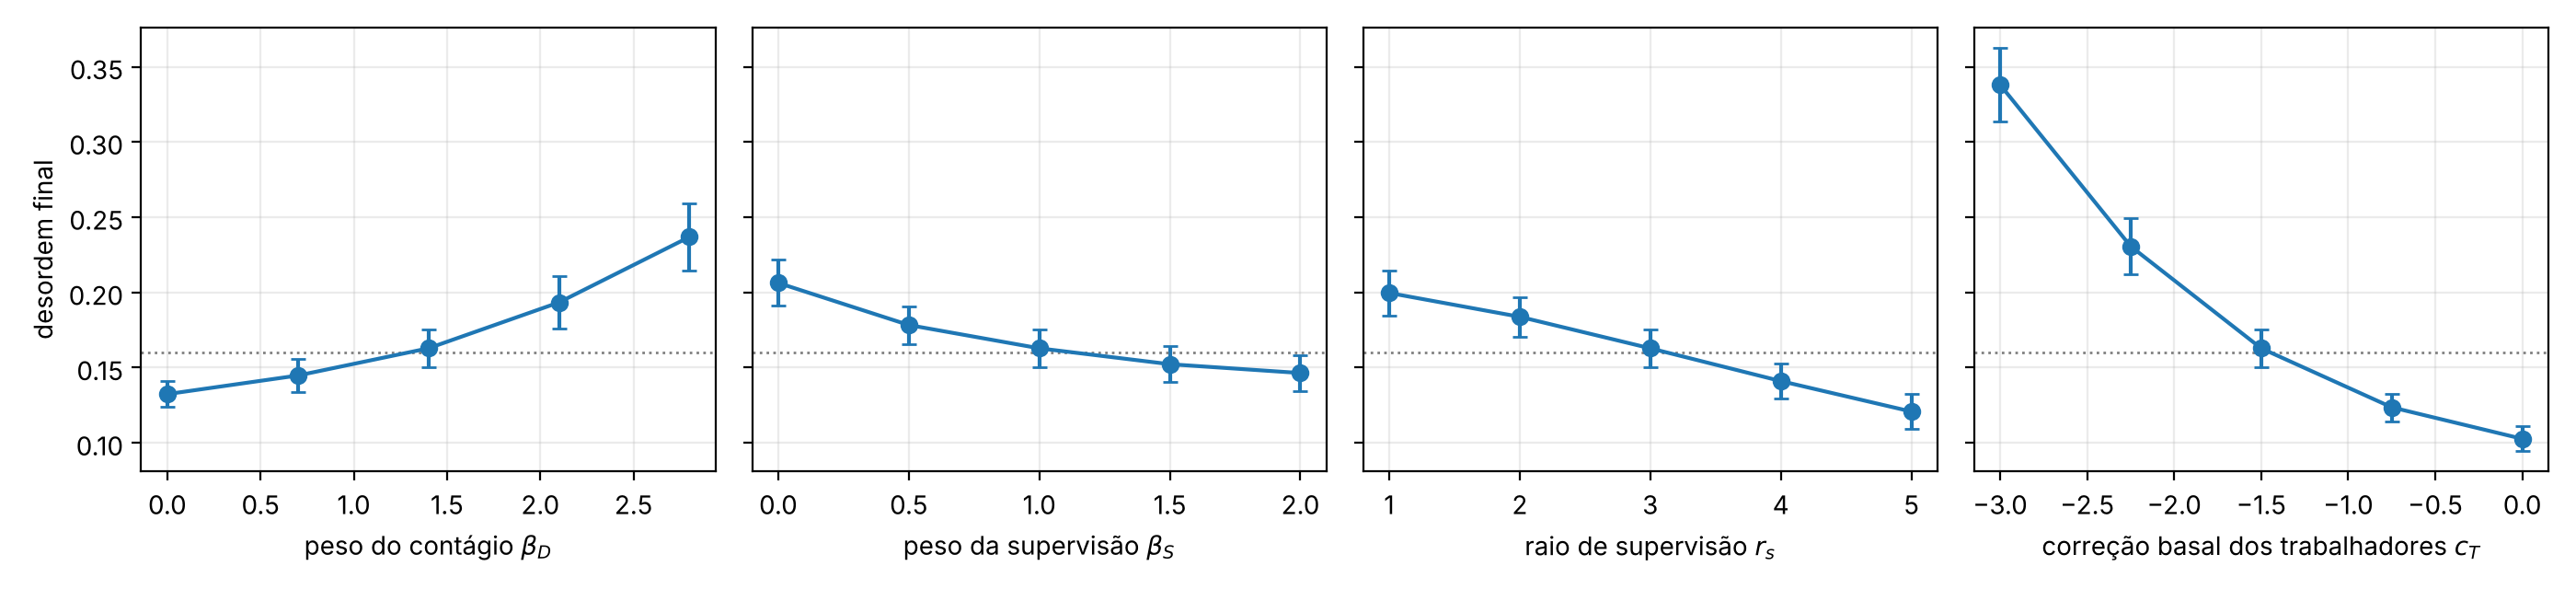
\includegraphics[width=\textwidth]{fig4_sensibilidade.png}\\[2pt]
  \small
  \begin{itemize}
    \item $c_T$ (correção basal) tem o maior efeito: 0,338 $\rightarrow$ 0,103 ($-70\%$), com retornos decrescentes.
    \item $r_s$ de 1 a 5: 0,200 $\rightarrow$ 0,121 ($-40\%$). $\beta_S$ de 0 a 2: 0,206 $\rightarrow$ 0,146 ($-29\%$), saturando.
    \item $\beta_D$ de 0 a 2,8: 0,132 $\rightarrow$ 0,237. Amplitudes: $c_T$ 0,235; $\beta_D$ 0,105; $r_s$ 0,079; $\beta_S$ 0,060.
  \end{itemize}
  \fonte{Política aleatória; média e IC 95\% de 10 sementes; linha pontilhada: cenário base (0,160).}
\end{frame}

\begin{frame}{Simulação e análise}{Políticas de movimento dos corretores}
  \centering
  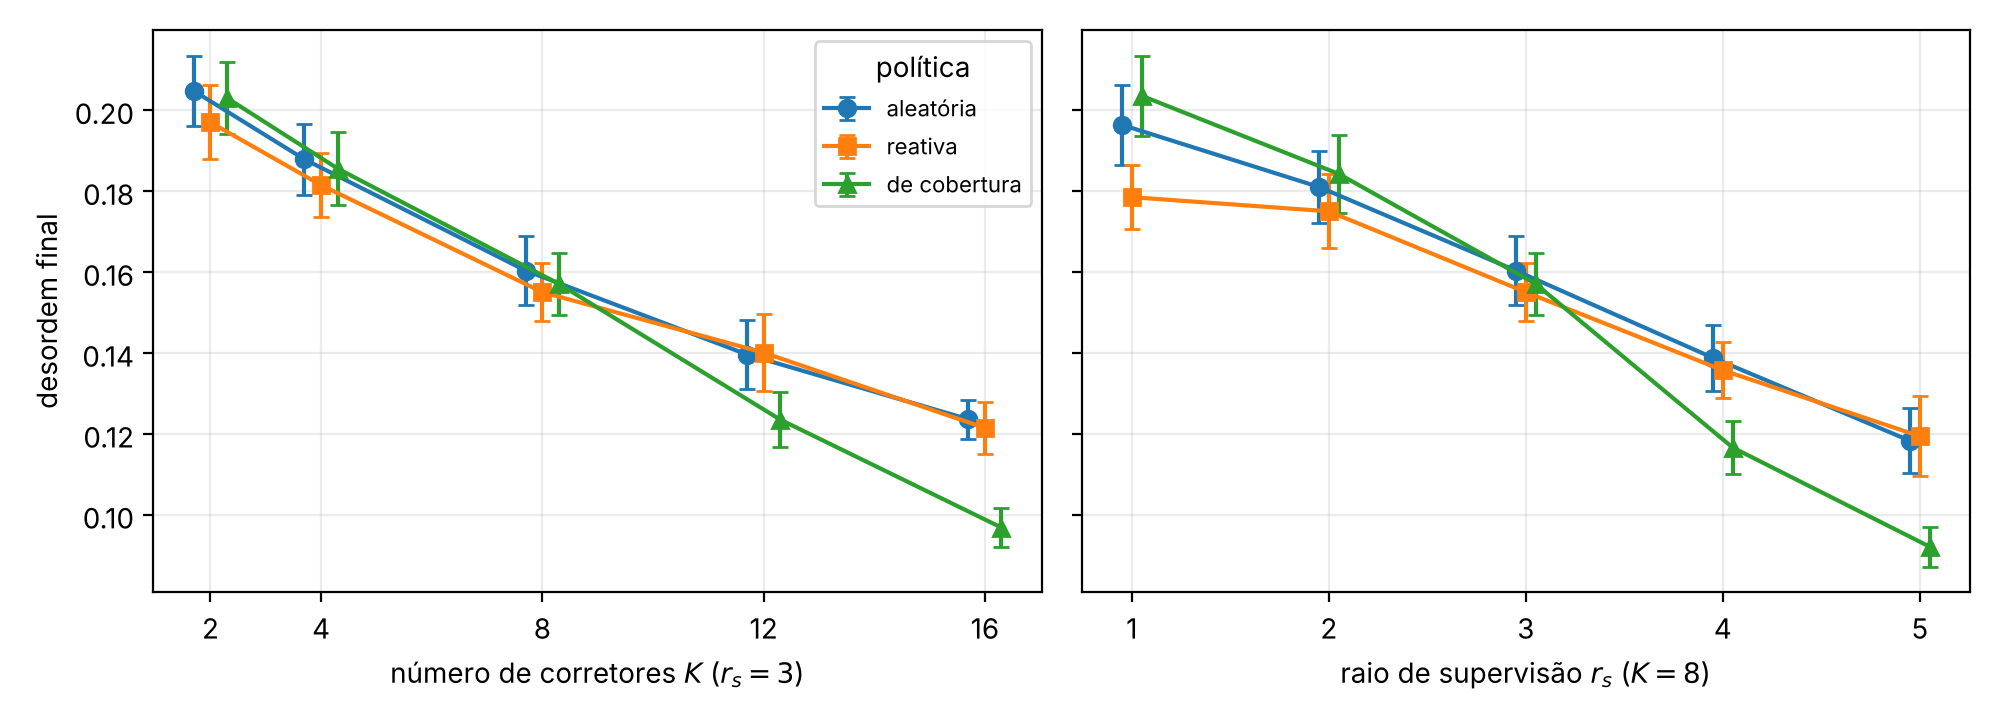
\includegraphics[width=0.72\textwidth]{fig7_politicas.png}\\[2pt]
  \footnotesize
  \begin{itemize}
    \item \textbf{Base ($K=8$, $r_s=3$):} 0,160, 0,155 e 0,157, indistinguíveis (IC $\pm0{,}011$).
    \item \textbf{Cobertura com supervisão ampla:} $K=16$: 0,097 contra 0,124 ($-0{,}027\pm0{,}007$); $r_s=5$: 0,092 contra 0,118. A grade supervisionada passa de 59\% para até 87\% com $K=16$.
    \item \textbf{Reativa:} sem ganho consistente (só $r_s=1$: 0,179 contra 0,196).
  \end{itemize}
  \fonte{20 sementes por ponto; média e IC 95\%.}
\end{frame}

\begin{frame}{Simulação e análise}{Síntese: quanto cada alavanca reduz a desordem}
  \centering\footnotesize
  \begin{tabular}{@{}lccc@{}}
    \toprule
    Alavanca & Variação & Desordem & vs.\ base (0,160) \\
    \midrule
    Moral média $\bar M$ & 0,50 $\to$ 0,75 & 0,076 & $-52\%$ \\
    Pressão $P$ & 0,50 $\to$ 0,25 & 0,120 & $-25\%$ \\
    Correção basal $c_T$ & $-1{,}5\to-1{,}0$ & 0,132 & $-18\%$ \\
    Corretores $K$ & 8 $\to$ 12 & 0,140 & $-13\%$ \\
    Raio $r_s$ & 3 $\to$ 4 & 0,139 & $-13\%$ \\
    Corretores $K$, rota de cobertura & 8 $\to$ 16 & 0,097 & $-40\%$ \\
    Raio $r_s$, rota de cobertura & 3 $\to$ 5 & 0,092 & $-43\%$ \\
    \midrule
    Moral média $\bar M$ (piora) & 0,50 $\to$ 0,25 & 0,328 & $+104\%$ \\
    Pressão $P$ (piora) & 0,50 $\to$ 0,75 & 0,213 & $+33\%$ \\
    \bottomrule
  \end{tabular}
  \fonte{20 sementes por linha; IC 95\% de $\pm0{,}004$ a $\pm0{,}015$.}
\end{frame}

% =====================================================================
\section{Conclusão}
% =====================================================================

\begin{frame}{Conclusão}{Resposta à pergunta e alavancas}
  \begin{block}{Resposta}
    \small Os desvios convergem para um único patamar (0,160 da área no base), que nunca chega a zero. Moral e facilidade de corrigir pesam mais do que pressão e supervisão. A escalada só ocorre com moral muito baixa (0,33 com $\bar M=0{,}25$) ou contágio acima do limiar ($\beta_D$ entre 3 e 5).
  \end{block}
  \begin{columns}[T]
    \begin{column}{0.52\textwidth}
      \begin{exampleblock}{Alavancas, em ordem de efeito}
        \footnotesize
        \begin{enumerate}
          \item \textbf{Moral:} treinamento, reconhecimento e feedback ($-52\%$)
          \item \textbf{Pressão:} evitar medidas que a elevem ($-25\%$ com $P=0{,}25$)
          \item \textbf{Facilitar a correção:} coletores e identificação clara ($-18\%$)
          \item \textbf{Alcance da supervisão} e rota de cobertura ($-40\%$ a $-43\%$)
          \item \textbf{Não deixar desordem acumular:} $\beta_D\le2{,}8$ $\Rightarrow$ desordem $<0{,}24$
        \end{enumerate}
      \end{exampleblock}
    \end{column}
    \begin{column}{0.44\textwidth}
      \begin{alertblock}{Alavancas fracas ou condicionais}
        \footnotesize
        \begin{itemize}
          \item Rota dos corretores: iguais com $K=8$ e $r_s=3$; cobertura só ganha 0,02 a 0,03 com supervisão ampla
          \item Rota reativa: sem ganho consistente
          \item Picos de pressão: +67\% por 50 passos e volta ao base em $\approx$45 passos
        \end{itemize}
      \end{alertblock}
    \end{column}
  \end{columns}
\end{frame}

\begin{frame}{Conclusão}{Limitações e próximos passos}
  \begin{columns}[T]
    \begin{column}{0.48\textwidth}
      \begin{alertblock}{Limitações}
        \begin{itemize}
          \item Parâmetros da literatura, sem calibração com dados da área: valores absolutos ilustrativos
          \item $P$ e $M$ constantes em cada execução
          \item Só descarte de resíduo comum; sem desvios médios e graves
          \item Grade homogênea, sem layout, turnos ou rotinas
          \item De 4 a 20 sementes por ponto: diferenças abaixo de $\approx$0,01 são ruído
        \end{itemize}
      \end{alertblock}
    \end{column}
    \begin{column}{0.48\textwidth}
      \begin{block}{Próximos passos}
        \begin{itemize}
          \item Tornar $P$ e $M$ variáveis no tempo, com os atrasos de R2, B1, B2 e B3
          \item Calibrar com registros de desvios da área
          \item Incluir layout da planta e desvios de maior gravidade
        \end{itemize}
      \end{block}
    \end{column}
  \end{columns}
\end{frame}

\begin{frame}[plain]
  \vfill\centering
  \begin{beamercolorbox}[sep=10pt, center, rounded=true, shadow=true]{title}
    \usebeamerfont{title}Obrigado!\\[2pt]
    \usebeamerfont{subtitle}Código: \texttt{github.com/Rafioio/Pensamento-Sistemico-em-Engenharia-Trabalho-Pratico}
  \end{beamercolorbox}
  \vfill
\end{frame}

\begin{frame}{Referências}
  \tiny
  \bibliographystyle{plainnat}
  \bibliography{../relatorio/referencias}
\end{frame}

\end{document}